% FORMAT AND PACKAGES
% {
\documentclass[a4paper]{article}
\usepackage{a4wide,amssymb,epsfig,latexsym,multicol,array,hhline,fancyhdr}
\usepackage{vntex}
\usepackage{amsmath}
\usepackage{lastpage}
\usepackage[lined,boxed,commentsnumbered]{algorithm2e}
\usepackage{enumerate}
\usepackage{xcolor}
\usepackage{graphicx}							% Standard graphics package
\usepackage{array}
\usepackage{enumitem}
\usepackage{listings}
\usepackage{tabularx, caption}
\usepackage{multirow}
\usepackage{multicol}
\usepackage{rotating}
\usepackage{graphics}
\usepackage{geometry}
\usepackage{setspace}
\usepackage{algorithm}
\usepackage{algorithmic}
\usepackage{epsfig}
\usepackage{tikz}
\usetikzlibrary{shapes.geometric, arrows, positioning}
\usepackage{xfrac}
\usepackage{bm}
\usepackage[colorlinks]{hyperref}
\usepackage{placeins}
\usepackage{graphicx}      % để dùng \includegraphics
\usepackage{float}         % để dùng [H] cho figure
\usepackage{tcolorbox}     % để vẽ khung tcolorbox

\usepackage{pdfpages}      % hỗ trợ trích trang từ PDF (nếu cần)
% \usepackage[acronym,toc]{glossaries}
% \usepackage[symbols,nogroupskip,nonumberlist]{glossaries-extra}
\usepackage[
 sort=none,% no sorting or indexing required
 abbreviations,% create list of abbreviations
 symbols,% create list of symbols
 stylemods,style=list, % set the default glossary style
 nogroupskip, nonumberlist, nomain
]{glossaries-extra}
\lstset{
    language=Python,
    basicstyle=\ttfamily\small,
    keywordstyle=\color{blue},
    commentstyle=\color{gray},
    stringstyle=\color{red},
    numbers=left,
    numberstyle=\tiny\color{gray},
    stepnumber=1,
    numbersep=10pt,
    frame=single,
    breaklines=true,
    tabsize=4,
    showstringspaces=false
}

% FORMATTING
% {
\DeclareMathOperator{\arccot}{arccot}
\captionsetup[table]{name=Table}
\captionsetup[figure]{name=Figure}
\newenvironment{Description}{\list{}{%
    \let\makelabel\descriptionlabel    % this comes from the original description environment
    \setlength{\rightmargin}{\leftmargin}% this comes from the original quote environment
    \setlength{\labelwidth}{0pt}%          this is new
    }}{\endlist}

\hypersetup{urlcolor=blue,linkcolor=black,citecolor=black,colorlinks=true} 
\usetikzlibrary{arrows,snakes,backgrounds}
\definecolor{mathblue}{RGB}{0,114,188}
% \makeatletter  \def\m@th{\mathsurround\z@\color{mathblue}} \makeatother
% \everymath{\color{mathblue}}
% \setmathfont[Color=000000]{Arial}
%\usepackage{pstcol} 								% PSTricks with the standard color package
\newtheorem{theorem}{{\bf Theorem}}
\newtheorem{property}{{\bf Property}}
\newtheorem{proposition}{{\bf Proposition}}
\newtheorem{corollary}[proposition]{{\bf Corollary}}
\newtheorem{lemma}[proposition]{{\bf Lemma}}

\AtBeginDocument{\renewcommand{\listfigurename}{List of Figures}}
\AtBeginDocument{\renewcommand{\listtablename}{List of Tables}}
\AtBeginDocument{\renewcommand*\contentsname{Contents}}
\AtBeginDocument{\renewcommand*\refname{References}}
%\usepackage{fancyhdr}

\setlength{\headheight}{40pt}
\pagestyle{fancy}
\fancyhead{} % clear all header fields
\fancyhead[L]{
 \begin{tabular}{rl}
    \begin{picture}(25,15)(0,0)
    \put(0,-8){
\includegraphics[width=8mm, height=8mm]{hcmut.png}}
    %\put(0,-8){\epsfig{width=10mm,figure=hcmut.eps}}
   \end{picture}&
	%
\includegraphics[width=8mm, height=8mm]{hcmut.png} & %
	\begin{tabular}{l}
		\textbf{\bf \ttfamily Trường đại học Bách khoa - DHQG TPHCM}\\
		\textbf{\bf \ttfamily Khoa khoa học và kỹ thuật máy tính}
	\end{tabular} 	
 \end{tabular}
}
\fancyhead[R]{
	\begin{tabular}{l}
		\tiny \bf \\
		\tiny \bf 
	\end{tabular}  }
\fancyfoot{} % clear all footer fields
\fancyfoot[L]{\scriptsize \ttfamily Bài tập lớn môn Kho dữ liệu và Hệ hỗ trợ quyết định}
\fancyfoot[R]{\scriptsize \ttfamily Page {\thepage}/\pageref{LastPage}}
\renewcommand{\headrulewidth}{0.3pt}
\renewcommand{\footrulewidth}{0.3pt}

\setcounter{secnumdepth}{4}
\setcounter{tocdepth}{4}

\makeatletter
\newcounter {subsubsubsection}[subsubsection]
\renewcommand\thesubsubsubsection{\thesubsubsection .\@alph\c@subsubsubsection}
\newcommand\subsubsubsection{\@startsection{subsubsubsection}{4}{\z@}%
                                     {-3.25ex\@plus -1ex \@minus -.2ex}%
                                     {1.5ex \@plus .2ex}%
                                     {\normalfont\normalsize\bfseries}}
\newcommand*\l@subsubsubsection{\@dottedtocline{3}{10.0em}{4.1em}}
\newcommand*{\subsubsubsectionmark}[1]{}
% \def\m@th{\mathsurround\z@\color{mathblue}}
\makeatother
% }
% }

% ACRONYMS & SYMBOLS
% {
% \makeglossaries
\setabbreviationstyle{long-short}
\newabbreviation{ode}{ODE}{(First-Order) Ordinary Differential Equation}
\newabbreviation{ivp}{IVP}{Initial-Value Problem}
\newabbreviation{lte}{LTE}{Local Truncation Error}
\newabbreviation{ds}{DS}{Dynamical System}
\newabbreviation{fig}{Fig.}{Figure}
\newabbreviation{tab}{Tab.}{Table}
\newabbreviation{sys}{Sys.}{System of Equations}
\newabbreviation{eq}{Eq.}{Equation}
\newabbreviation{eg}{e.g.}{For Example}
\newabbreviation{ie}{i.e.}{That Is}
% \glsnoexpandfields
\glsxtrnewsymbol[description = {Set of natural numbers}]{natural}{\ensuremath{\mathbb{N}}}
\glsxtrnewsymbol[description = {Set of real numbers}]{real}{\ensuremath{\mathbb{R}}}
\glsxtrnewsymbol[description = {Set of positive real numbers}]{real_positive}{\ensuremath{\mathbb{R}^+}}

% }

% DOCUMENT
\begin{document}

% TITLE PAGE
\begin{titlepage}
\begin{center}
TRƯỜNG ĐẠI HỌC BÁCH KHOA - ĐHQG TP.HCM \\
KHOA KHOA HỌC VÀ KỸ THUẬT MÁY TÍNH
\end{center}

\vspace{1cm}

\begin{figure}[h!]
\begin{center}

\includegraphics[width=4cm]{hcmut.png}
\end{center}
\end{figure}

\vspace{1cm}


\begin{center}
\begin{tabular}{c}
\multicolumn{1}{l}{\textbf{{\Large KHO DỮ LIỆU VÀ HỆ HỖ TRỢ QUYẾT ĐỊNH (CO4031)}}}\\
~~\\
\hline
\\
\multicolumn{1}{l}{\textbf{{\Large Báo cáo bài tập lớn}}}\\
\\
\textbf{\textit{{\Huge Olist E-commerce}}}\\
\textbf{\textit{{\Large Xây dựng kho dữ liệu và hệ hỗ trợ quyết định}}}\\
\\
\hline
\end{tabular}
\end{center}

\vspace{1cm}

\begin{table}[h]
\centering
    \begin{tabular}{rl}
    \hspace{2 cm}\textbf{Giảng viên phụ trách}:
    & Đỗ Thanh Thái\\
    & \\[10pt]
    \textbf{Sinh viên thực hiện}: & .................................... - MSSV: ................\\
    & .................................... - MSSV: ................\\
    & .................................... - MSSV: ................\\
    \end{tabular}
\end{table}
\begin{center}
{\footnotesize HỌC KỲ 261 -- NĂM HỌC 2026--2027}
\end{center}
\end{titlepage}


\section{Phương pháp thực hiện}
Đề tài sử dụng hai hướng tiếp cận:
\begin{itemize}
    \item \textbf{Phân khúc khách hàng:} dùng K-Means để nhóm các hồ sơ RFM có hành vi mua tương đồng.
    \item \textbf{Dự đoán giao trễ:} dùng Logistic Regression, Random Forest và LightGBM để phân loại đơn hàng.
\end{itemize}

\subsection{Thuật toán phân cụm K-Means}
\noindent\textbf{Giới thiệu bài toán}\par
Khách hàng có sự khác biệt về thời điểm mua, tần suất và mức chi tiêu. Phân khúc theo hành vi giúp doanh nghiệp lựa chọn cách chăm sóc, giữ chân hoặc tái kích hoạt phù hợp với từng nhóm.

Khảo sát 93.358 khách hàng từ các đơn đã giao có tiền hàng dương cho thấy khoảng 97\% chỉ mua một đơn; Recency và Monetary vẫn phân bố khác nhau như Hình~\ref{fig:rfm-exploration}. Vì vậy, đề tài kết hợp cả ba chỉ số RFM để phân nhóm, thay vì chỉ xét tần suất mua.

\begin{figure}[htbp]
\centering
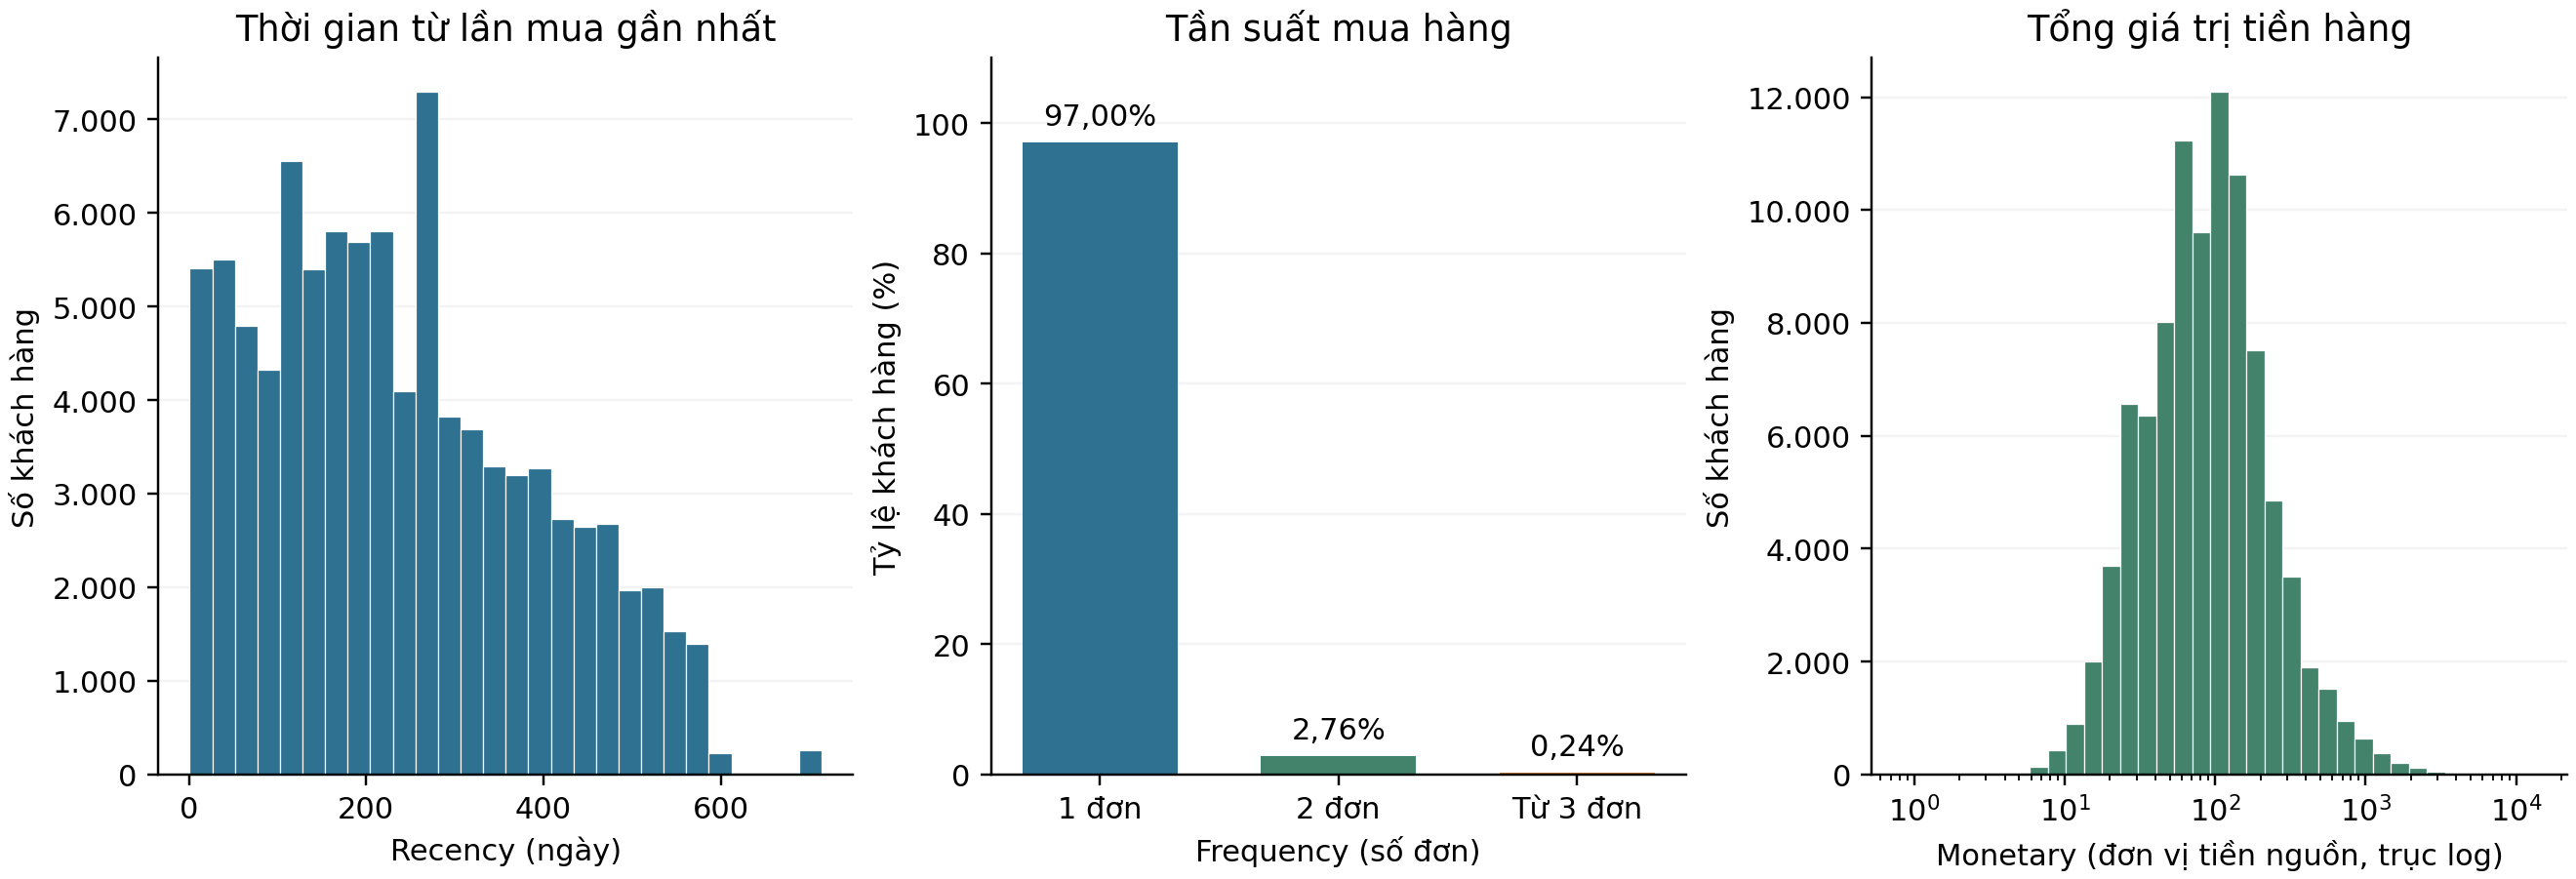
\includegraphics[width=\textwidth]{assets/rfm_exploration.png}
\caption{Khảo sát RFM trên dữ liệu nguồn Olist.}
\label{fig:rfm-exploration}
\end{figure}

\subsubsection{Giới thiệu thuật toán}
K-Means là thuật toán học không giám sát, chia dữ liệu thành $K$ cụm mà không cần nhãn định trước. Mỗi cụm được đại diện bởi một tâm (centroid), tính bằng trung bình các vector thuộc cụm. Thuật toán lặp giữa gán điểm vào tâm gần nhất và cập nhật tâm cụm \cite{kmeansTheory}.

Mục tiêu là tạo các nhóm có đặc trưng gần nhau trong không gian biểu diễn. Kết quả là mã cụm của từng khách hàng; tên nhóm nghiệp vụ được xác định sau khi phân tích đặc điểm của cụm.

\subsubsection{Hàm mục tiêu của K-Means}
Thuật toán tối thiểu hóa tổng bình phương khoảng cách trong cụm (WCSS, hay inertia):
\[
J=\sum_{k=1}^{K}\sum_{\mathbf{x}_i\in C_k}
\|\mathbf{x}_i-\boldsymbol{\mu}_k\|_2^2,
\]
Trong đó, $C_k$ là cụm thứ $k$, $\boldsymbol{\mu}_k$ là tâm cụm và $\mathbf{x}_i$ là vector đặc trưng của khách hàng. Bình phương khoảng cách làm các điểm nằm xa tâm đóng góp nhiều hơn vào mục tiêu. WCSS nhỏ hơn thể hiện cụm chặt hơn trên cùng dữ liệu; chỉ số này thường giảm khi tăng $K$.

\subsubsection{Nguyên lý hoạt động của thuật toán}
\begin{enumerate}
    \item \textbf{Khởi tạo:} xác định $K$ tâm ban đầu.
    \item \textbf{Gán cụm:} đưa mỗi điểm vào cụm có tâm gần nhất theo khoảng cách Euclid:
    \[
    c_i=\underset{k\in\{1,\ldots,K\}}{\operatorname{arg\,min}}
    \|\mathbf{x}_i-\boldsymbol{\mu}_k\|_2^2.
    \]
    \item \textbf{Cập nhật tâm:} tính lại trung bình các điểm thuộc mỗi cụm không rỗng:
    \[
    \boldsymbol{\mu}_k=\frac{1}{|C_k|}\sum_{\mathbf{x}_i\in C_k}\mathbf{x}_i.
    \]
    \item \textbf{Lặp:} tiếp tục đến khi tâm thay đổi không đáng kể hoặc đạt giới hạn số lần lặp.
\end{enumerate}
Hai bước gán cụm và cập nhật tâm giúp giảm hoặc giữ nguyên hàm mục tiêu trong quá trình lặp. Kết quả phụ thuộc khởi tạo và không bảo đảm tối ưu toàn cục; nhiều lần khởi tạo giúp giảm sự phụ thuộc vào một phương án ban đầu.

\subsubsection{Lựa chọn số cụm}
Hai phương pháp thường dùng để hỗ trợ lựa chọn $K$ gồm:
\begin{itemize}
    \item \textbf{Elbow Method:} chọn vùng mà WCSS bắt đầu giảm chậm khi tăng $K$.
    \item \textbf{Silhouette Score:} đánh giá độ kết dính trong cụm và mức tách biệt giữa các cụm.
\end{itemize}
Cần kết hợp các chỉ số với khả năng diễn giải và mục tiêu nghiệp vụ.

\subsubsection{Ưu điểm của thuật toán K-Means}
\begin{itemize}
    \item Nguyên lý đơn giản, dễ triển khai.
    \item Phù hợp với dữ liệu đặc trưng số như RFM.
    \item Thuận tiện tóm tắt và so sánh các nhóm khách hàng.
\end{itemize}

\subsubsection{Hạn chế của thuật toán K-Means}
\begin{itemize}
    \item Cần xác định trước số cụm $K$.
    \item Nhạy cảm với khởi tạo, ngoại lệ và thang đo.
    \item Hạn chế khi các cụm có hình dạng phức tạp hoặc độ phân tán khác nhau.
\end{itemize}

\subsubsection{Ứng dụng trong bài toán phân khúc khách hàng}
K-Means sử dụng ba chỉ số Recency, Frequency và Monetary để nhận diện các nhóm hành vi mua hàng. Tên nhóm được đặt sau phân cụm dựa trên RFM gốc, làm cơ sở đề xuất hoạt động chăm sóc phù hợp.

\subsection{Dự đoán nguy cơ giao hàng trễ}
\noindent\textbf{Giới thiệu bài toán}\par
Giao hàng đúng hẹn là một yếu tố gắn với trải nghiệm mua sắm. Nhận diện sớm đơn có nguy cơ giao trễ giúp doanh nghiệp chủ động theo dõi, điều phối và trao đổi với khách hàng \cite{hartman2026}.

Khảo sát 95.824 đơn Olist đã giao và có đánh giá cho thấy \textbf{53,72\% đơn giao trễ nhận 1 sao}, trong khi tỷ lệ này ở nhóm đúng hạn là \textbf{6,61\%} (Hình~\ref{fig:delivery-review}). Mối liên hệ này tạo động lực xây dựng mô hình phân loại giao trễ; thống kê mô tả chưa khẳng định quan hệ nhân quả.

\begin{figure}[htbp]
\centering
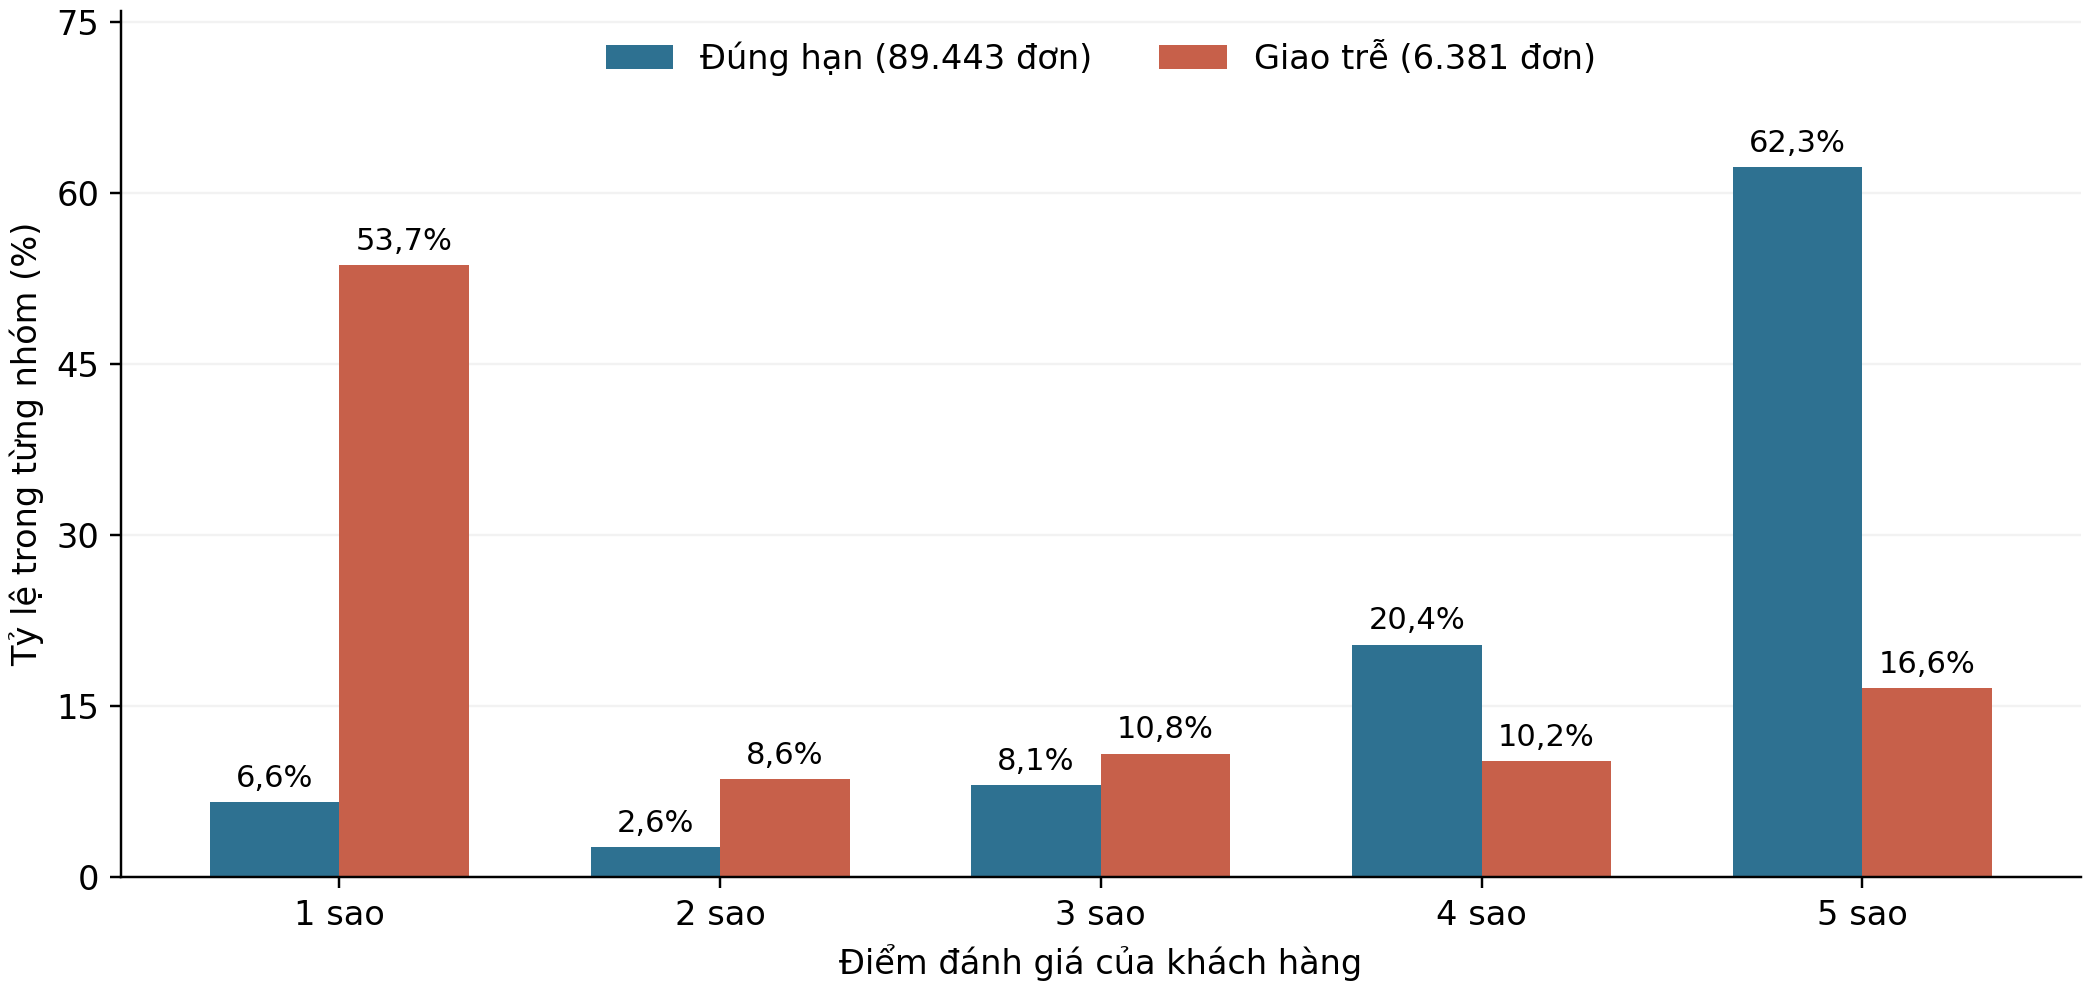
\includegraphics[width=0.95\textwidth]{assets/review_delivery_distribution.png}
\caption{Phân bố điểm đánh giá trong từng nhóm giao hàng. Chỉ xét đơn đã giao, đủ ngày giao và ngày hẹn; mỗi đơn giữ đánh giá có thời điểm trả lời sớm nhất.}
\label{fig:delivery-review}
\end{figure}

\subsubsection{Phát biểu bài toán và hướng tiếp cận}
Đây là bài toán phân loại nhị phân ở cấp đơn hàng:
\begin{itemize}
    \item \textbf{Đầu vào:} thông tin đơn hàng, sản phẩm, vận chuyển và lịch sử người bán.
    \item \textbf{Đầu ra:} nhãn giao trễ ($y=1$) hoặc đúng hạn ($y=0$), kèm điểm dự đoán.
    \item \textbf{Phương pháp:} so sánh Logistic Regression, Random Forest và LightGBM.
\end{itemize}
Thông tin đầu vào phải có sẵn tại thời điểm dự đoán. Ngày giao thực tế chỉ dùng tạo nhãn; lịch sử người bán chỉ lấy từ kết quả đã biết trước đó. Do mất cân bằng lớp, cần xem xét khả năng phát hiện đơn trễ bên cạnh Accuracy \cite{hartman2026}.

\subsubsection{Logistic Regression}
\noindent\textbf{1. Giới thiệu}\par
Logistic Regression là thuật toán phân loại sử dụng hàm sigmoid để ước lượng xác suất một đối tượng thuộc lớp dương. Trong đề tài, lớp dương là đơn giao trễ. Mô hình đóng vai trò \textit{baseline tuyến tính}, làm cơ sở so sánh với Random Forest và LightGBM.

\noindent\textbf{2. Ý tưởng và cơ chế}\par
Với vector đặc trưng $\mathbf{x}$, mô hình kết hợp tuyến tính các biến rồi chuyển thành xác suất:
\[
z=\beta_0+\boldsymbol{\beta}^{T}\mathbf{x},\qquad
p(y=1\mid\mathbf{x})=\sigma(z)=\frac{1}{1+e^{-z}}.
\]
Trong đó, $\beta_0$ là hệ số chặn và $\boldsymbol{\beta}$ là vector trọng số. Quan hệ tuyến tính áp dụng cho log-odds:
\[
\log\frac{p}{1-p}=\beta_0+\boldsymbol{\beta}^{T}\mathbf{x}.
\]
Khi giữ các biến khác không đổi, dấu của hệ số thể hiện chiều liên hệ với log-odds giao trễ. Điểm dự đoán được so sánh với một ngưỡng để gán nhãn; ngưỡng thấp hơn thường làm tăng số đơn được cảnh báo.

\noindent\textbf{3. Hàm mục tiêu}\par
Mô hình tối thiểu hóa mất mát logarit nhị phân, tương đương cực đại hóa log-likelihood. Với điều chuẩn $L_2$, có thể viết mục tiêu dưới dạng:
\[
\mathcal{J}=-\sum_{i=1}^{n}
\left[y_i\log p_i+(1-y_i)\log(1-p_i)\right]
+\frac{\lambda}{2}\|\boldsymbol{\beta}\|_2^2.
\]
Ở đây, $p_i$ là xác suất dự đoán của đơn thứ $i$ và $\lambda$ điều khiển mức điều chuẩn. Thành phần $L_2$ hạn chế trọng số quá lớn. Trong triển khai, $C$ là tham số nghịch với mức điều chuẩn; $C$ nhỏ tương ứng điều chuẩn mạnh hơn \cite{logisticTheory}.

\noindent\textbf{4. Ưu điểm}\par
\begin{itemize}
    \item Cấu trúc đơn giản, thuận tiện làm mô hình cơ sở.
    \item Trọng số hỗ trợ diễn giải chiều liên hệ giữa đặc trưng và log-odds.
    \item Cho đầu ra dạng xác suất để điều chỉnh ngưỡng cảnh báo.
    \item Điều chuẩn giúp kiểm soát độ lớn trọng số và hạn chế quá khớp.
\end{itemize}

\noindent\textbf{5. Hạn chế}\par
\begin{itemize}
    \item Giới hạn khi ranh giới giữa hai lớp có dạng phi tuyến phức tạp.
    \item Không tự xây dựng tương tác giữa các biến đầu vào.
    \item Cần xử lý thang đo; đa cộng tuyến làm hệ số khó diễn giải riêng lẻ.
    \item Kết quả phân loại chịu ảnh hưởng của phân bố lớp và ngưỡng dự đoán.
\end{itemize}



\subsubsection{Random Forest}
\noindent\textbf{1. Giới thiệu}\par
Random Forest là phương pháp học tổ hợp kết hợp nhiều cây quyết định. Một cây đơn phân chia dữ liệu bằng các điều kiện trên đặc trưng, nhưng dễ thay đổi khi tập huấn luyện thay đổi. Việc tổng hợp nhiều cây có yếu tố ngẫu nhiên giúp giảm phương sai và sự phụ thuộc vào một cây riêng lẻ.

\noindent\textbf{2. Ý tưởng và cơ chế}\par
Hai cơ chế chính tạo sự đa dạng giữa các cây gồm:
\begin{itemize}
    \item \textbf{Bagging:} mỗi cây học trên một mẫu bootstrap được lấy có hoàn lại từ tập huấn luyện. Một đơn có thể xuất hiện nhiều lần hoặc không được chọn trong mẫu của cây đó.
    \item \textbf{Ngẫu nhiên hóa đặc trưng:} tại mỗi nút, chỉ xét một tập con đặc trưng để tìm phép chia, hạn chế các cây cùng ưu tiên một biến.
\end{itemize}
Trong triển khai sử dụng ở đề tài, điểm giao trễ là trung bình xác suất của các cây \cite{forestTheory}:
\[
\widehat{p}(y=1\mid\mathbf{x})=\frac{1}{T}\sum_{t=1}^{T}p_t(y=1\mid\mathbf{x}),
\]
trong đó $T$ là số cây và $p_t$ là xác suất do cây thứ $t$ cung cấp. Nhãn cuối được xác định bằng ngưỡng trên điểm trung bình này.

\noindent\textbf{3. Tiêu chí phân chia}\par
Mỗi cây sử dụng độ không thuần Gini để đánh giá mức pha trộn nhãn tại một nút:
\[
G(t)=1-p_0(t)^2-p_1(t)^2,
\]
trong đó $p_0(t),p_1(t)$ là tỷ lệ hai lớp. Nút chỉ chứa một lớp có Gini bằng không. Với hai nút con trái và phải, mức giảm độ không thuần là:
\[
\Delta G=G(t)-\frac{n_L}{n_t}G(t_L)-\frac{n_R}{n_t}G(t_R),
\]
trong đó $n_t,n_L,n_R$ lần lượt là số mẫu tại nút cha và hai nút con.

\noindent\textbf{4. Xây dựng cây và tổng hợp dự đoán}\par
\begin{enumerate}
    \item Tạo mẫu bootstrap cho từng cây.
    \item Chọn tập con đặc trưng, tìm phép chia có mức giảm Gini lớn nhất trong các phương án xét.
    \item Lặp phân chia đến khi đạt điều kiện dừng, chẳng hạn số mẫu tối thiểu tại lá hoặc không còn phép chia phù hợp.
    \item Đưa đơn cần dự đoán qua từng cây, lấy trung bình xác suất rồi gán nhãn.
\end{enumerate}
Các cây được xây dựng độc lập với nhau về quá trình học, nên có thể huấn luyện song song. Việc tìm phép chia là tối ưu cục bộ tại từng nút, không phải tối ưu toàn bộ rừng trong một bước.

\noindent\textbf{5. Ưu điểm}\par
\begin{itemize}
    \item Học được quan hệ phi tuyến và tương tác giữa các đặc trưng.
    \item Giảm phương sai so với một cây quyết định đơn.
    \item Ít phụ thuộc chuẩn hóa thang đo ở bước học cây.
    \item Có thể khai thác nhiều lõi xử lý để xây dựng các cây song song.
\end{itemize}

\noindent\textbf{6. Hạn chế}\par
\begin{itemize}
    \item Tốn bộ nhớ và chi phí dự đoán khi rừng có nhiều cây lớn.
    \item Khó diễn giải tổng thể hơn một cây đơn.
    \item Bagging không tự khắc phục mất cân bằng lớp.
    \item Độ quan trọng đặc trưng không chứng minh quan hệ nhân quả.
\end{itemize}



\subsubsection{LightGBM}
\noindent\textbf{1. Giới thiệu}\par
LightGBM là phương pháp gradient boosting trên cây quyết định, phù hợp để khai thác quan hệ phi tuyến trong dữ liệu dạng bảng. Các cây được xây dựng tuần tự: mỗi cây mới bổ sung một phần điều chỉnh nhằm giảm hàm mất mát của tổ hợp hiện tại.

\noindent\textbf{2. Ý tưởng và cơ chế}\par
Hai cơ chế nổi bật của LightGBM gồm:
\begin{itemize}
    \item \textbf{Histogram:} gom giá trị liên tục vào các khoảng, tổng hợp thống kê trong từng khoảng để giảm số ngưỡng cần xét khi chia nút.
    \item \textbf{Phát triển theo lá (leaf-wise):} ưu tiên tách lá có mức giảm hàm mục tiêu lớn nhất, thay vì mở rộng đồng loạt theo độ sâu \cite{lightgbmTheory}.
\end{itemize}
Phát triển theo lá có thể tạo cây không cân đối. Vì vậy, số lá và số mẫu tối thiểu trong lá cần được kiểm soát để hạn chế quá khớp.

\noindent\textbf{3. Hàm mục tiêu và cập nhật mô hình}\par
Với bài toán nhị phân, LightGBM sử dụng mất mát logarit để đánh giá điểm dự đoán. Tổ hợp được cập nhật theo công thức:
\[
F_m(\mathbf{x})=F_{m-1}(\mathbf{x})+\eta f_m(\mathbf{x}),
\]
trong đó $F_{m-1}$ là điểm trước cập nhật, $f_m$ là cây mới và $\eta$ là tốc độ học. Xác suất giao trễ được tính bởi:
\[
p_m(y=1\mid\mathbf{x})=\frac{1}{1+e^{-F_m(\mathbf{x})}}.
\]
Tốc độ học nhỏ giảm đóng góp của từng cây; cần cân nhắc cùng số vòng boosting để đạt mức khớp dữ liệu phù hợp.

\noindent\textbf{4. Ưu điểm}\par
\begin{itemize}
    \item Biểu diễn được quan hệ phi tuyến và tương tác giữa các biến.
    \item Histogram hỗ trợ giảm chi phí tìm phép chia và lưu trữ.
    \item Tổ hợp được cải thiện theo từng giai đoạn dựa trên hàm mất mát.
    \item Có nhiều tham số để kiểm soát độ phức tạp của cây.
\end{itemize}

\noindent\textbf{5. Hạn chế}\par
\begin{itemize}
    \item Có thể quá khớp khi cây nhiều lá hoặc số vòng boosting lớn.
    \item Tốc độ học, số cây và số lá có tác động kết hợp, cần điều chỉnh phù hợp.
    \item Khó giải thích toàn bộ tổ hợp cây bằng các quy tắc đơn giản.
    \item Vẫn cần đánh giá cách cân bằng dữ liệu và ngưỡng phân loại.
\end{itemize}



\subsection{Kỹ thuật cân bằng dữ liệu}
Các đơn giao trễ là lớp thiểu số trong dữ liệu Olist. Để tăng số mẫu đại diện cho lớp này khi huấn luyện, đề tài sử dụng hai kỹ thuật sinh mẫu tổng hợp: SMOTE và SMOTENC.

\subsubsection{SMOTE}
\noindent\textbf{1. Giới thiệu}\par
SMOTE (Synthetic Minority Over-sampling Technique) tạo thêm mẫu thuộc lớp thiểu số bằng nội suy, thay vì chỉ sao chép các mẫu hiện có \cite{smoteTheory}.

\noindent\textbf{2. Cơ chế tạo mẫu}\par
Với mẫu thiểu số $\mathbf{x}_i$ và một láng giềng cùng lớp $\mathbf{x}_j$, mẫu mới được xác định bởi:
\[
\mathbf{x}_{\mathrm{new}}=\mathbf{x}_i+\alpha(\mathbf{x}_j-\mathbf{x}_i),
\qquad \alpha\in[0,1].
\]
Hệ số $\alpha$ được chọn ngẫu nhiên; mẫu mới nằm trên đoạn nối hai vector. Quy trình gồm:
\begin{enumerate}
    \item Chọn mẫu thuộc lớp thiểu số và tìm các láng giềng cùng lớp.
    \item Chọn một láng giềng, nội suy để tạo mẫu mới.
    \item Lặp đến khi đạt số mẫu yêu cầu.
\end{enumerate}

\noindent\textbf{3. Ưu điểm}\par
\begin{itemize}
    \item Tăng số mẫu lớp thiểu số mà không chỉ lặp lại dữ liệu.
    \item Thuận tiện áp dụng trong quy trình huấn luyện phân loại.
\end{itemize}

\noindent\textbf{4. Hạn chế}\par
\begin{itemize}
    \item Có thể sinh mẫu tại vùng chồng lấn hoặc gần ngoại lệ.
    \item Khoảng cách láng giềng phụ thuộc thang đo; nội suy các cột one-hot có thể tạo giá trị phân số.
\end{itemize}

\subsubsection{SMOTENC}
\noindent\textbf{1. Giới thiệu}\par
SMOTENC (Synthetic Minority Over-sampling Technique for Nominal and Continuous) mở rộng SMOTE cho dữ liệu có cả biến số và biến phân loại \cite{smotencTheory}. Trong bài toán giao trễ, danh mục sản phẩm là biến phân loại cần xử lý riêng.

\noindent\textbf{2. Cơ chế tạo mẫu}\par
\begin{enumerate}
    \item Khai báo các cột phân loại và tìm láng giềng cho mẫu thiểu số trong không gian hỗn hợp.
    \item Nội suy phần đặc trưng số để tạo giá trị mới.
    \item Chọn giá trị phân loại xuất hiện nhiều nhất trong các láng giềng, thay vì nội suy mã danh mục.
\end{enumerate}
Cách xử lý này giữ giá trị danh mục dưới dạng nhãn hợp lệ trước bước mã hóa cho mô hình.

\noindent\textbf{3. Ưu điểm}\par
\begin{itemize}
    \item Phân biệt vai trò của biến số và biến phân loại khi sinh mẫu.
    \item Tránh tạo giá trị phân số cho danh mục theo cách nội suy trực tiếp one-hot.
\end{itemize}

\noindent\textbf{4. Hạn chế}\par
\begin{itemize}
    \item Cần khai báo đúng biến phân loại; không dành cho dữ liệu chỉ có biến phân loại.
    \item Vẫn chịu ảnh hưởng của láng giềng, thang đo và vùng chồng lấn giữa các lớp.
\end{itemize}

\section{Xây dựng và cấu hình mô hình}
\subsection{Mô hình phân khúc khách hàng}
\subsubsection{Xây dựng và tiền xử lý RFM}
Chỉ sử dụng đơn đã giao, có tiền hàng lớn hơn không và thuộc khoảng năm được chọn. Các chỉ số gồm:
\begin{itemize}
    \item \textbf{Recency:} số ngày từ lần mua gần nhất đến ngày tham chiếu; mốc tham chiếu là ngày mua cuối của tập dữ liệu cộng một ngày.
    \item \textbf{Frequency:} số đơn khác nhau của khách hàng.
    \item \textbf{Monetary:} tổng tiền hàng, không gồm phí vận chuyển.
\end{itemize}
Frequency và Monetary được chặn tại P99 rồi biến đổi logarit; Recency được đảo chiều kết hợp logarit. Ba biến sau đó được chuẩn hóa bằng StandardScaler.

\begin{figure}[htbp]
\centering
\begin{tikzpicture}[node distance=0.45cm, box/.style={draw,rounded corners,align=center,text width=10cm,minimum height=0.85cm},>=stealth]
\node[box] (a) {Đơn đã giao trong khoảng năm được chọn};
\node[box,below=of a] (b) {Tổng hợp theo khách hàng: Recency, Frequency, Monetary};
\node[box,below=of b] (c) {Chặn P99 của F/M; biến đổi logarit và đảo R; chuẩn hóa};
\node[box,below=of c] (d) {K-Means với K=4};
\node[box,below=of d] (e) {Diễn giải bằng RFM gốc và gán nhãn nghiệp vụ};
\draw[->] (a)--(b); \draw[->] (b)--(c); \draw[->] (c)--(d); \draw[->] (d)--(e);
\end{tikzpicture}
\caption{Quy trình phân khúc khách hàng bằng RFM và K-Means.}
\label{fig:rfm-process}
\end{figure}

\subsubsection{Cấu hình K-Means}
\begin{itemize}
    \item \texttt{n\_clusters=4}: tạo bốn nhóm phục vụ diễn giải nghiệp vụ.
    \item \texttt{random\_state=42}: hỗ trợ tái lập trên cùng dữ liệu và môi trường.
    \item \texttt{n\_init=10}: khởi tạo mười lần, giữ kết quả có inertia nhỏ nhất.
\end{itemize}
$K=4$ là lựa chọn triển khai, chưa được xác nhận tối ưu. Mô hình được huấn luyện lại theo khoảng năm; mã cụm có thể thay đổi giữa các lần chạy.

\subsection{Mô hình dự đoán giao hàng trễ}
\subsubsection{Dữ liệu đầu vào và định nghĩa nhãn}
Dữ liệu Olist được tổng hợp thành một dòng cho mỗi đơn hàng. Nhãn được xác định theo ngày lịch:
\begin{itemize}
    \item $y=1$: ngày giao thực tế sau ngày giao dự kiến.
    \item $y=0$: giao trong hoặc trước ngày dự kiến.
\end{itemize}
Đơn thiếu thông tin xác định nhãn không được mặc định gán là đúng hạn.

\subsubsection{Xây dựng đặc trưng}
Mô hình sử dụng mười đặc trưng gồm chín biến số và một biến phân loại, chi tiết tại Bảng~\ref{tab:late-features}.

\begin{table}[htbp]
\centering
\small
\begin{tabularx}{\textwidth}{|c|p{5.4cm}|p{1.4cm}|X|}
\hline
\textbf{STT} & \textbf{Đặc trưng} & \textbf{Kiểu} & \textbf{Ý nghĩa và cách xác định} \\ \hline
1 & \texttt{distance\_km} & Số & Khoảng cách địa lý người bán--khách hàng (km); lấy giá trị lớn nhất trong các dòng hàng của đơn. \\ \hline
2 & \texttt{freight\_value} & Số & Tổng phí vận chuyển của các dòng hàng trong đơn, theo đơn vị tiền nguồn. \\ \hline
3 & \texttt{shipping\_days\_estimated} & Số & Số ngày từ thời điểm mua đến ngày hẹn giao; tính từ chênh lệch thời gian và làm tròn đến hai chữ số thập phân. \\ \hline
4 & \texttt{order\_weekday} & Số & Thứ trong tuần tại thời điểm mua, mã hóa từ 0 (thứ Hai) đến 6 (Chủ nhật). \\ \hline
5 & \texttt{order\_purchase\_month} & Số & Tháng mua hàng, nhận giá trị từ 1 đến 12. \\ \hline
6 & \texttt{item\_physical\_score} & Số & Tổng chỉ số khối lượng nhân chiều dài, chiều rộng và chiều cao, chia 1.000, tính trên các dòng hàng của đơn. \\ \hline
7 & \texttt{delayed\_orders\_by\_seller} & Số & Số đơn giao trễ trong lịch sử đã biết của người bán trước thời điểm mua đơn cần dự đoán. \\ \hline
8 & \texttt{delay\_rate\_percent\_by\_seller} & Số & Tỷ lệ đơn giao trễ trong lịch sử đã biết của người bán, biểu diễn theo phần trăm. \\ \hline
9 & \texttt{seller\_avg\_delay\_days} & Số & Trung bình chênh lệch ngày giao thực tế so với ngày hẹn trong lịch sử đã biết; giá trị âm thể hiện giao sớm. \\ \hline
10 & \texttt{product\_category\_name} & Phân loại & Danh mục sản phẩm xuất hiện nhiều nhất trong đơn; được mã hóa one-hot trước khi đưa vào mô hình. \\ \hline
\end{tabularx}
\caption{Mười đặc trưng đầu vào của mô hình dự đoán giao hàng trễ, trước khi mã hóa danh mục sản phẩm.}
\label{tab:late-features}
\end{table}

Lịch sử người bán chỉ dùng kết quả thuộc tập huấn luyện đã biết trước lúc mua đơn cần dự đoán; đơn nhiều người bán lấy trung bình các thống kê. Ngày giao thực tế của chính đơn không làm đặc trưng. Sau one-hot danh mục sản phẩm, số cột có thể lớn hơn mười.

\subsubsection{Tổ chức dữ liệu cho DSS}
Module huấn luyện đọc các bảng fact và dimension trong PostgreSQL sau ETL. Từ phép chia phân tầng năm fold với seed 42, hệ thống dùng fold 4 đã chọn trong thực nghiệm trước. Trong phần train, 20\% đơn thật được giữ riêng để hiệu chỉnh sigmoid với tỷ lệ trễ tự nhiên. Phần còn lại dùng để fit bộ tiền xử lý, tính lịch sử seller và huấn luyện ba mô hình. Với mỗi đơn, lịch sử seller chỉ gồm kết quả đã biết trước thời điểm mua.

\subsubsection{Cân bằng dữ liệu bằng SMOTE và SMOTENC}
Tập huấn luyện được cân bằng thành 20.000 đơn hàng, gồm 10.000 đơn đúng hạn và 10.000 đơn giao trễ. Mẫu tổng hợp chỉ được tạo cho lớp giao trễ trong tập huấn luyện; tập kiểm thử giữ các đơn thật.
\begin{itemize}
    \item \textbf{SMOTE -- Logistic Regression:} mã hóa danh mục sản phẩm bằng one-hot trước khi sinh mẫu.
    \item \textbf{SMOTENC -- Random Forest và LightGBM:} chuẩn hóa biến số và khai báo \texttt{product\_category\_name} là biến phân loại khi sinh mẫu; sau đó mã hóa cho mô hình.
\end{itemize}
Cả hai kỹ thuật sử dụng \texttt{k\_neighbors=5} và \texttt{random\_state=42}.

\begin{figure}[H]
\centering
\begin{tikzpicture}[node distance=0.4cm, box/.style={draw,rounded corners,align=center,text width=10.5cm,minimum height=0.85cm},>=stealth]
\node[box] (a) {Làm sạch dữ liệu Olist; xây dựng mười đặc trưng và nhãn giao trễ};
\node[box,below=of a] (b) {Tách fold 4 để kiểm thử; dành 20\% phần train để hiệu chỉnh};
\node[box,below=of b] (c) {Mã hóa đặc trưng; cân bằng tập huấn luyện thành 20.000 dòng};
\node[box,below=of c] (d) {Huấn luyện Logistic Regression, Random Forest và LightGBM};
\node[box,below=of d] (e) {Giữ cố định mô hình nền; fit sigmoid trên tập hiệu chỉnh};
\node[box,below=of e] (f) {Đánh giá trên toàn bộ fold 4; so sánh Brier score trước và sau hiệu chỉnh};
\draw[->] (a)--(b); \draw[->] (b)--(c); \draw[->] (c)--(d);
\draw[->] (d)--(e); \draw[->] (e)--(f);
\end{tikzpicture}
\caption{Quy trình huấn luyện và đánh giá ba mô hình dự đoán giao hàng trễ.}
\label{fig:late-process}
\end{figure}

\subsubsection{Cấu hình ba thuật toán}
Cả ba mô hình sử dụng seed 42 và ngưỡng phân loại cuối 0,4. Cấu hình cụ thể được trình bày trong các bảng dưới đây.

\noindent\textbf{Logistic Regression}\par
Các biến số được chuẩn hóa; tập huấn luyện được cân bằng bằng SMOTE.

\begin{table}[H]
\centering
\small
\caption{Các tham số của Logistic Regression trong đề tài.}
\label{tab:lr-parameters}
\begin{tabularx}{\textwidth}{|p{3.7cm}|X|}
\hline
\textbf{Tham số} & \textbf{Mô tả} \\ \hline
\texttt{C} & Nghịch đảo mức điều chuẩn; giá trị nhỏ tăng mức điều chuẩn.\par\smallskip Trong đề tài: \texttt{0.001}. \\ \hline
\texttt{penalty} & Phạt bình phương độ lớn trọng số.\par\smallskip Trong đề tài: \texttt{l2}. \\ \hline
\texttt{solver} & Phương pháp tối ưu trọng số.\par\smallskip Trong đề tài: \texttt{lbfgs}. \\ \hline
\texttt{max\_iter} & Giới hạn số vòng tối ưu; không mặc định bảo đảm hội tụ.\par\smallskip Trong đề tài: \texttt{2000}. \\ \hline
\texttt{class\_weight} & Không bổ sung trọng số lớp; dữ liệu đã được cân bằng.\par\smallskip Trong đề tài: \texttt{None}. \\ \hline
\texttt{random\_state} & Giá trị hạt giống được thiết lập trong cấu hình.\par\smallskip Trong đề tài: \texttt{42}. \\ \hline
\end{tabularx}
\end{table}

\noindent\textbf{Random Forest}\par
Tập huấn luyện được cân bằng bằng SMOTENC.

\begin{table}[H]
\centering
\small
\caption{Các tham số của Random Forest trong đề tài.}
\label{tab:rf-parameters}
\begin{tabularx}{\textwidth}{|p{3.7cm}|X|}
\hline
\textbf{Tham số} & \textbf{Mô tả} \\ \hline
\texttt{n\_estimators} & Số cây quyết định trong rừng.\par\smallskip Trong đề tài: \texttt{300}. \\ \hline
\texttt{max\_features} & Tỷ lệ đặc trưng được xem xét khi tìm phép chia.\par\smallskip Trong đề tài: \texttt{0.7}. \\ \hline
\texttt{max\_depth} & Không đặt giới hạn trực tiếp cho độ sâu cây.\par\smallskip Trong đề tài: \texttt{None}. \\ \hline
\texttt{min\_samples\_leaf} & Số mẫu tối thiểu tại một nút lá.\par\smallskip Trong đề tài: \texttt{1}. \\ \hline
\texttt{criterion} & Tiêu chí độ không thuần để đánh giá phép chia.\par\smallskip Trong đề tài: \texttt{gini}. \\ \hline
\texttt{bootstrap} & Sử dụng lấy mẫu có hoàn lại cho mỗi cây.\par\smallskip Trong đề tài: \texttt{True}. \\ \hline
\end{tabularx}
\end{table}

\noindent\textbf{LightGBM}\par
Tập huấn luyện được cân bằng bằng SMOTENC.

\begin{table}[H]
\centering
\small
\caption{Các tham số của LightGBM trong đề tài.}
\label{tab:lgbm-parameters}
\begin{tabularx}{\textwidth}{|p{3.7cm}|X|}
\hline
\textbf{Tham số} & \textbf{Mô tả} \\ \hline
\texttt{n\_estimators} & Số vòng boosting.\par\smallskip Trong đề tài: \texttt{100}. \\ \hline
\texttt{learning\_rate} & Mức đóng góp của mỗi cây mới.\par\smallskip Trong đề tài: \texttt{0.03}. \\ \hline
\texttt{num\_leaves} & Số lá tối đa của mỗi cây.\par\smallskip Trong đề tài: \texttt{63}. \\ \hline
\texttt{min\_child\_samples} & Số mẫu tối thiểu dùng để kiểm soát các lá nhỏ.\par\smallskip Trong đề tài: \texttt{100}. \\ \hline
\texttt{colsample\_bytree} & Tỷ lệ đặc trưng lấy mẫu cho mỗi cây.\par\smallskip Trong đề tài: \texttt{0.7}. \\ \hline
\texttt{reg\_lambda} & Không bổ sung phạt L2 lên trọng số lá trong cấu hình này.\par\smallskip Trong đề tài: \texttt{0}. \\ \hline
\end{tabularx}
\end{table}

\subsubsection{Ngưỡng phân loại cuối}
Cả ba mô hình gán nhãn giao trễ khi điểm dự đoán từ 0,4 trở lên. Ngưỡng được chốt sau đối chiếu trên tập kiểm thử; giới hạn của cách lựa chọn này được nêu trong phần hạn chế thực nghiệm.

\section{Kết quả thực nghiệm và đánh giá}
\subsection{Phân khúc khách hàng}
Kết quả dưới đây được tổng hợp từ 93.350 khách hàng Olist, không lọc năm; ngày tham chiếu RFM là 30/08/2018. Kết quả chưa được đối soát với lần chạy DW theo khoảng năm người dùng chọn.

Bảng~\ref{tab:kmeans-medians} trình bày trung vị RFM gốc của từng cụm. Recency tính bằng ngày, Frequency bằng số đơn và Monetary theo đơn vị tiền nguồn.

\begin{table}[H]
\centering
\caption{Giá trị RFM trung vị của từng cụm khách hàng.}
\label{tab:kmeans-medians}
\begin{tabular}{c|r|r|r}
\hline
\textbf{Cluster} & \textbf{Recency} & \textbf{Frequency} & \textbf{Monetary} \\ \hline
0 & 180 & 1 & 44,90 \\
1 & 469 & 1 & 84,90 \\
2 & 200 & 2 & 182,10 \\
3 & 179 & 1 & 149,99 \\
\hline
\end{tabular}
\end{table}

Từ các giá trị trung vị, có thể diễn giải bốn nhóm như sau:
\begin{itemize}
    \item \textbf{Cụm 0 -- Khách chi tiêu thấp:} Monetary trung vị thấp nhất, 44,90; Frequency trung vị bằng 1.
    \item \textbf{Cụm 1 -- Khách lâu chưa mua:} Recency trung vị cao nhất, 469 ngày.
    \item \textbf{Cụm 2 -- Khách mua lại:} Frequency trung vị bằng 2 và Monetary trung vị đạt 182,10.
    \item \textbf{Cụm 3 -- Khách chi tiêu cao:} Monetary trung vị đạt 149,99, cao hơn cụm 0; hai cụm cùng có Frequency trung vị bằng 1.
\end{itemize}

\begin{figure}[htbp]
\centering
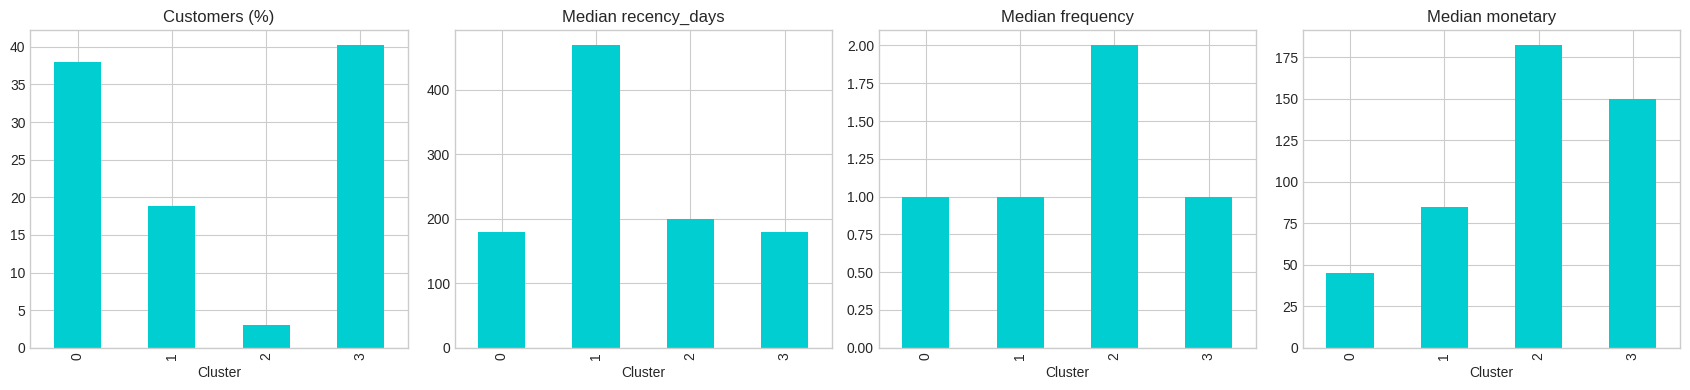
\includegraphics[width=\textwidth]{assets/kmeans4_profile.png}
\caption{Tỷ lệ khách hàng và trung vị RFM gốc theo bốn cụm. Recency tính bằng ngày, Frequency tính bằng số đơn, Monetary giữ đơn vị tiền nguồn.}
\label{fig:kmeans-profile}
\end{figure}

\begin{figure}[htbp]
\centering
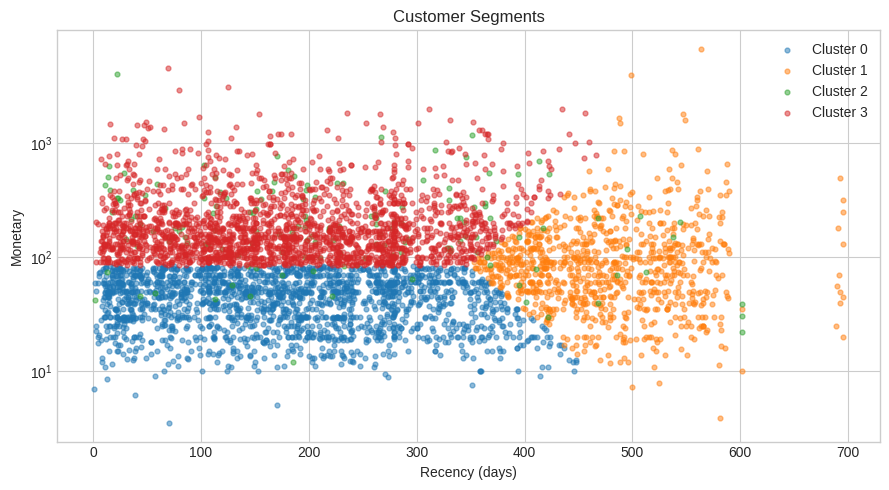
\includegraphics[width=0.95\textwidth]{assets/kmeans4_scatter.png}
\caption{Phân bố khách hàng theo Recency và Monetary trong thí nghiệm K=4. Monetary hiển thị trên thang logarit; hình lấy tối đa 5.000 khách để minh họa, còn mô hình sử dụng toàn bộ 93.350 khách. Hình là lát cắt hai chiều, không phải phép chiếu PCA.}
\label{fig:kmeans-scatter}
\end{figure}

\subsection{Dự đoán giao hàng trễ}
\subsubsection{Tiêu chí đánh giá}
Các chỉ số được tính cho lớp giao trễ:
\[
\mathrm{Precision}=\frac{\mathrm{TP}}{\mathrm{TP}+\mathrm{FP}},\qquad
\mathrm{Recall}=\frac{\mathrm{TP}}{\mathrm{TP}+\mathrm{FN}},\qquad
\mathrm{F1}=\frac{2\mathrm{TP}}{2\mathrm{TP}+\mathrm{FP}+\mathrm{FN}}.
\]
Trong đó, TP là cảnh báo đúng, FP là cảnh báo nhầm và FN là đơn trễ bị bỏ sót. Precision thể hiện độ tin cậy của cảnh báo, Recall thể hiện khả năng phát hiện và F1 kết hợp hai chỉ số.

\subsubsection{Kết quả trên tập kiểm thử}
Bảng và các hình trong mục này ghi lại thực nghiệm trước khi chuyển sang huấn luyện từ DW và hiệu chỉnh xác suất. Bảng~\ref{tab:late-test} trình bày kết quả trên cùng 2.596 đơn thật tại ngưỡng 0,4, đã đối chiếu bằng các mô hình được lưu.

\begin{table}[htbp]
\centering
\small
\begin{tabularx}{\textwidth}{|X|r|r|r|r|r|}
\hline
\textbf{Mô hình} & \textbf{Precision} & \textbf{Recall} & \textbf{F1} & \textbf{FP} & \textbf{FN} \\ \hline
Logistic Regression & 0,5198 & 0,9399 & 0,6694 & 1127 & 78 \\ \hline
Random Forest & 0,6976 & 0,6841 & 0,6908 & 385 & 410 \\ \hline
LightGBM & 0,6853 & 0,6995 & 0,6923 & 417 & 390 \\ \hline
\end{tabularx}
\caption{Kết quả nhận diện lớp giao trễ tại ngưỡng 0,4. FP là cảnh báo nhầm; FN là đơn trễ bị bỏ sót. Các chỉ số được làm tròn đến bốn chữ số thập phân.}
\label{tab:late-test}
\end{table}

\begin{figure}[htbp]
\centering
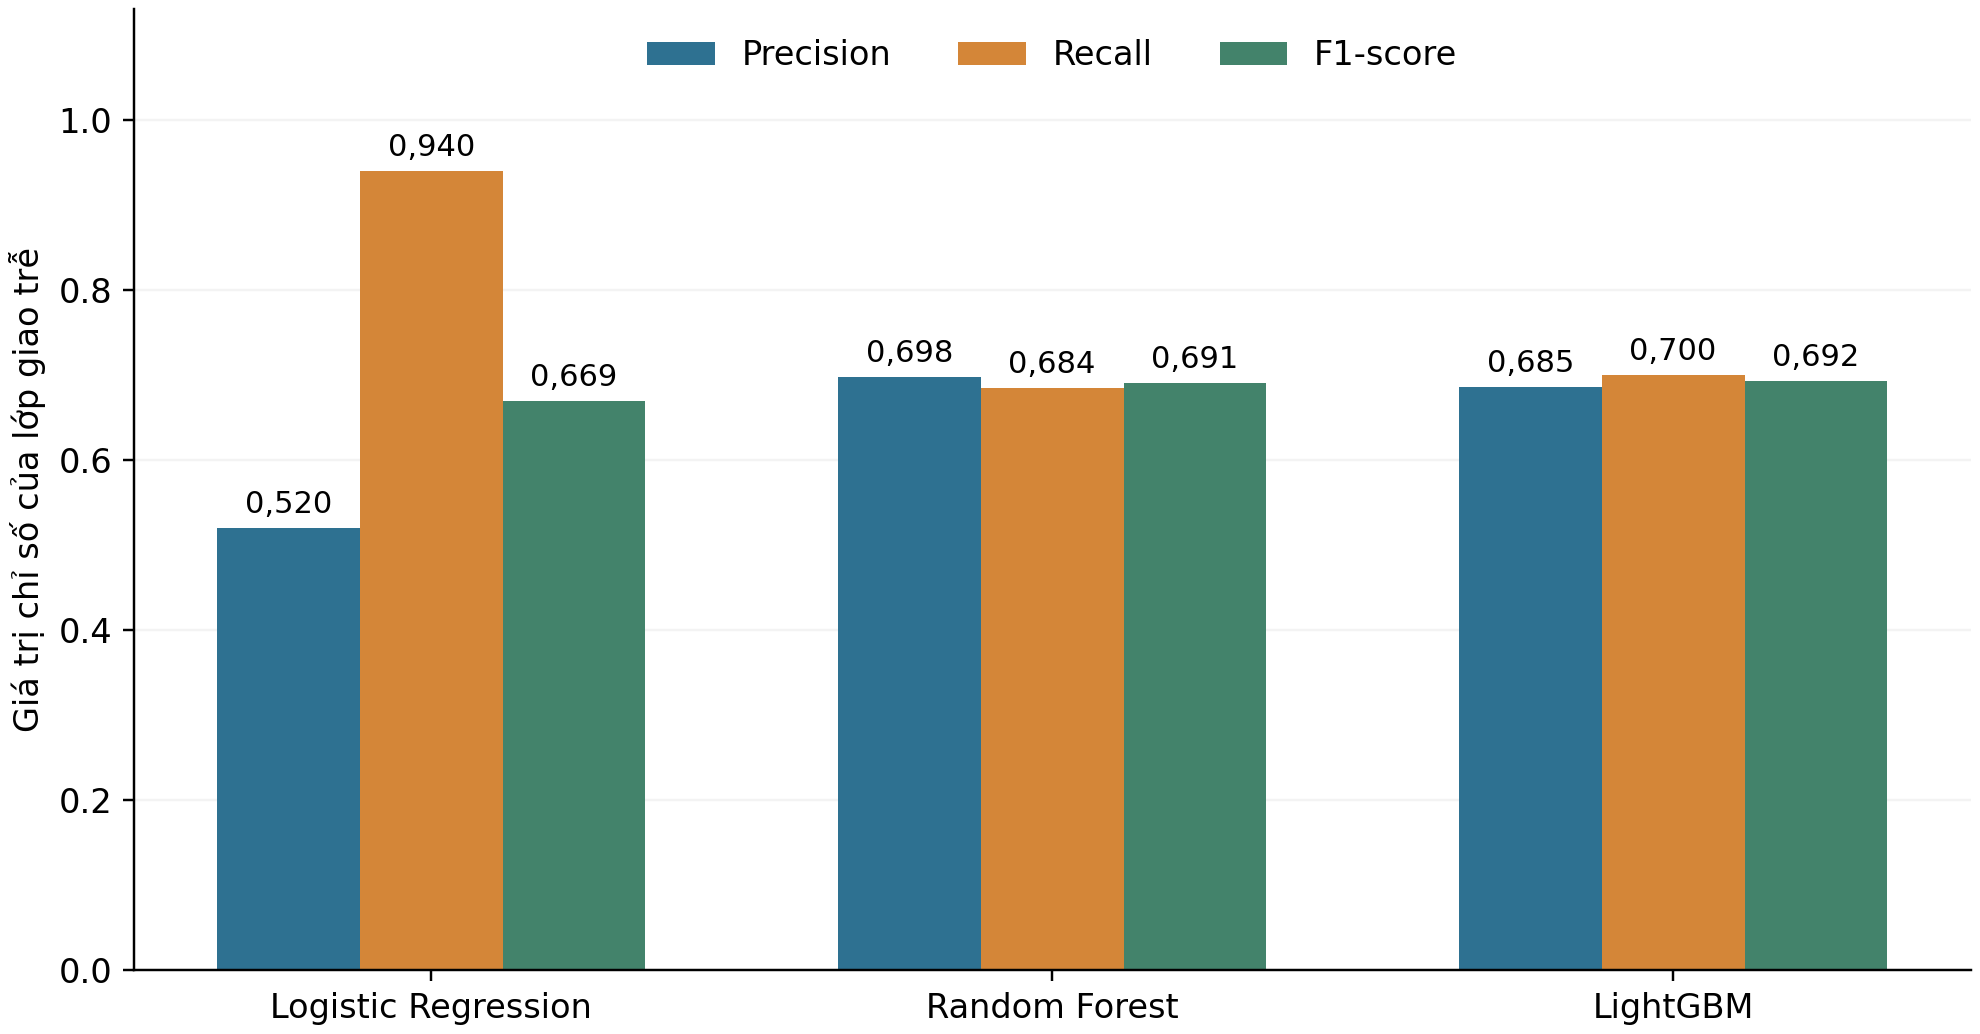
\includegraphics[width=0.95\textwidth]{assets/late_risk_metrics.png}
\caption{So sánh Precision, Recall và F1-score của lớp giao trễ trên cùng tập kiểm thử tại ngưỡng 0,4.}
\label{fig:late-metrics}
\end{figure}

\begin{itemize}
    \item \textbf{Logistic Regression:} Recall cao nhất (93,99\%), bỏ sót 78 đơn trễ nhưng cảnh báo nhầm 1.127 đơn.
    \item \textbf{Random Forest:} Precision cao nhất (69,76\%), với 385 cảnh báo nhầm và 410 đơn trễ bị bỏ sót.
    \item \textbf{LightGBM:} F1 cao nhất (0,6923), nhận diện thêm 20 đơn trễ nhưng cảnh báo nhầm thêm 32 đơn so với Random Forest.
\end{itemize}
Chênh lệch F1 giữa hai mô hình cây khoảng 0,0016, chưa chứng minh ưu thế ổn định trên dữ liệu khác.

\begin{figure}[htbp]
\centering
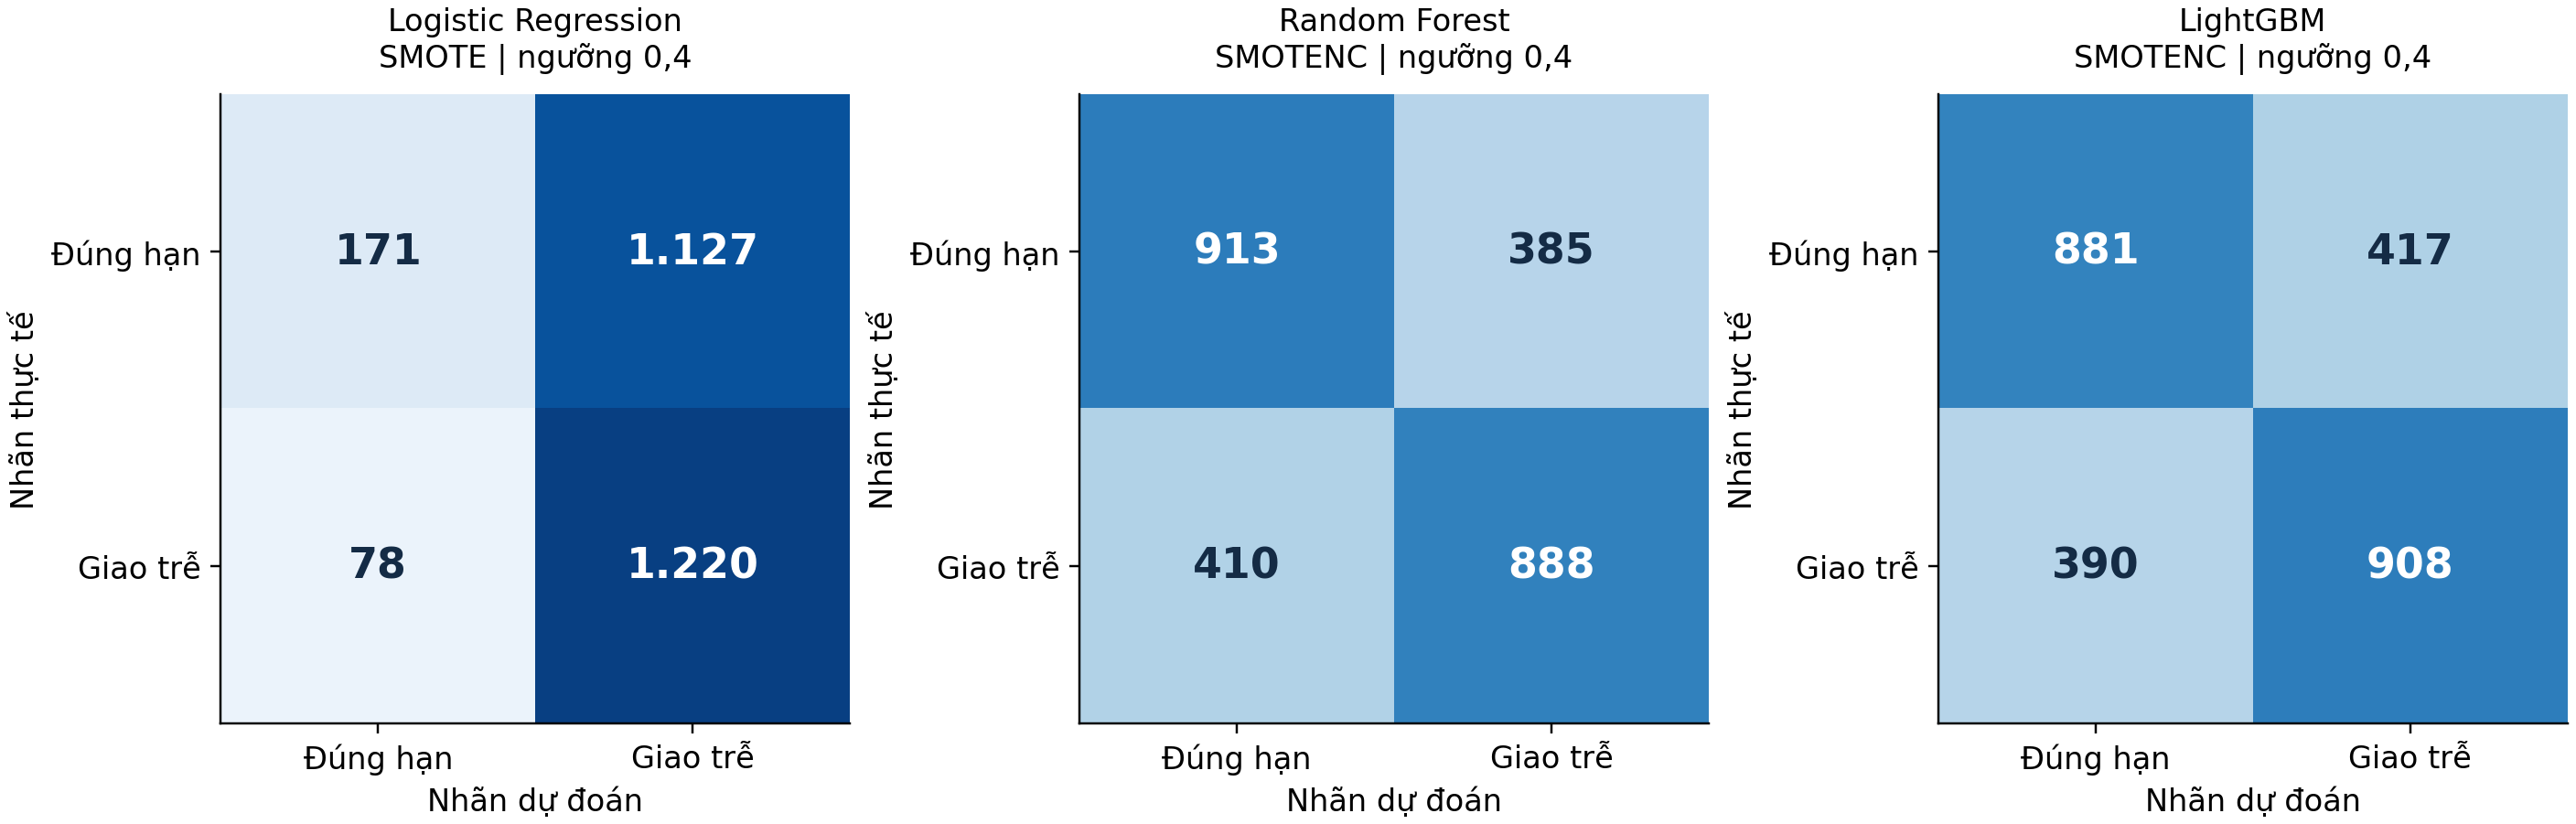
\includegraphics[width=\textwidth]{assets/late_risk_confusion.png}
\caption{Ma trận nhầm lẫn của ba mô hình tại ngưỡng 0,4. Hàng biểu diễn nhãn thực tế, cột biểu diễn nhãn dự đoán; mỗi ma trận có 2.596 đơn.}
\label{fig:late-confusion}
\end{figure}

\subsection{Hạn chế của thực nghiệm}
\begin{itemize}
    \item Tập kiểm thử 50:50 chưa phản ánh tỷ lệ giao trễ trong vận hành.
    \item Ngưỡng 0,4 được chốt sau khi xem kiểm thử; cần dữ liệu độc lập để xác nhận kết quả.
    \item Chưa đánh giá trên giai đoạn tương lai hoặc đo tác động kinh tế của các hành động can thiệp.
\end{itemize}

\section{Ứng dụng hỗ trợ quyết định}
\subsection{Chăm sóc khách hàng theo phân khúc}
Kết quả RFM và K-Means hỗ trợ chọn nhóm khách hàng cho hoạt động chăm sóc, giữ chân hoặc tái kích hoạt.

\subsection{Chọn đơn cần can thiệp}
Với mỗi đơn $i$, mô hình ước lượng xác suất giao trễ đã hiệu chỉnh $p_i$. Gọi $L$ là thiệt hại cơ sở, $w_i$ là hệ số nhóm khách K-Means, $e$ là tỷ lệ đơn vốn sẽ trễ mà can thiệp có thể giúp giao đúng hạn và $c$ là chi phí cho một lần can thiệp. Lợi ích ròng kỳ vọng của đơn là
\[
B_i = p_i L w_i e - c.
\]
Người vận hành nhập các giả định bằng cùng đơn vị tiền cho $L$ và $c$. DSS nối nhóm khách theo mã khách duy nhất từ kết quả phân cụm có trước ngày quyết định. Khách chưa phân nhóm nhận hệ số 1. Thống kê điểm review và tỷ lệ review 1--2 sao theo trạng thái giao giúp đối chiếu giả định, với mỗi đơn được tính cùng trọng số.

Mỗi mô hình xếp hạng riêng các đơn mua trong ngày theo $B_i$ giảm dần. Hệ thống chọn tối đa $N$ đơn có $B_i>0$ khi năng lực là $N$, hoặc chọn mọi đơn có lợi ích dương khi đủ năng lực. Khi hòa, ưu tiên xác suất trễ cao hơn rồi mã đơn tăng dần. Ngưỡng 0,4 chỉ dùng cho báo cáo phân loại trên điểm thô.

\subsection{Mô phỏng và phân tích độ nhạy}
CLI thử các tổ hợp chi phí, hiệu quả và năng lực. Với tập đơn được chọn $S$, tổng lợi ích là $\sum_{i\in S}B_i$ và số đơn trễ kỳ vọng tránh được là $\sum_{i\in S}p_i e$. Ví dụ minh họa với $p_i=0{,}20$, $L=100$, $w_i=1{,}5$, $e=0{,}5$, lợi ích gộp là 15 đơn vị tiền. Chi phí 10 cho lợi ích ròng 5; nếu chi phí tăng lên 15 thì đơn bị loại.

CLI xuất bảng theo đơn, người bán và tuyến vận chuyển. Đóng góp của đơn được chia đều giữa các người bán hoặc các tuyến riêng biệt. Biểu đồ tornado thay từng tham số $L$, $c$, $e$ ở mức $\pm20\%$, giới hạn $e$ trong $[0,1]$, rồi chọn lại đơn với cùng năng lực. Phần mềm đã được kiểm tra bằng dữ liệu tổng hợp. Cần chạy trên DW để báo cáo Brier score và kết quả kịch bản Olist; hiệu quả can thiệp thực tế cần được đo trong vận hành.

\section{Kết luận và hướng phát triển}
Đề tài hỗ trợ phân tích hành vi ở cấp khách hàng và nguy cơ giao trễ ở cấp đơn hàng. Hướng tiếp theo là đánh giá số cụm, kiểm thử trên dữ liệu tương lai và đo hiệu quả nghiệp vụ.

\begin{thebibliography}{9}
\bibitem{hartman2026} N. Hartman, S. Sarkar và A. Alhamadani, ``Learning to Predict Delivery Delays: An Analytical Study of Machine Learning and Oversampling Strategies,'' ICICT 2026, 2026. DOI: \url{https://doi.org/10.1145/3803291.3803322}.
\bibitem{kmeansTheory} Scikit-learn, ``Clustering: K-Means,'' \url{https://scikit-learn.org/stable/modules/clustering.html}.
\bibitem{logisticTheory} Scikit-learn, ``Linear Models: Logistic Regression,'' \url{https://scikit-learn.org/stable/modules/linear_model.html}.
\bibitem{forestTheory} Scikit-learn, ``Ensembles: Random Forests,'' \url{https://scikit-learn.org/stable/modules/ensemble.html}.
\bibitem{lightgbmTheory} LightGBM, ``Features,'' \url{https://lightgbm.readthedocs.io/en/stable/Features.html}.
\bibitem{smoteTheory} Imbalanced-learn, ``Over-sampling: Sample generation,'' \url{https://imbalanced-learn.org/stable/over_sampling.html}.
\bibitem{smotencTheory} Imbalanced-learn, ``SMOTENC,'' \url{https://imbalanced-learn.org/stable/references/generated/imblearn.over_sampling.SMOTENC.html}.
\end{thebibliography}
\end{document}
